\documentclass[11pt]{article}

\usepackage[margin=1in]{geometry}
\usepackage{amsmath,amssymb}
\usepackage{booktabs}
\usepackage{graphicx}
\usepackage{natbib}
\usepackage[hidelinks]{hyperref}
\usepackage{xcolor}

\newcommand{\todo}[1]{\textcolor{red}{[TODO: #1]}}

\title{Pulled, Moved, then Made:\\The Three-Phase Refill of Crypto Limit Order Books after Liquidity Sweeps}
\author{Joel Pulikkan\thanks{\todo{affiliation}. Email: joelpulikkan253@gmail.com. Code and processed results: \todo{repository URL}.}}
\date{\todo{date}}

\begin{document}
\maketitle

\begin{abstract}
When an aggressive order sweeps through several price levels of a limit order book, how does
the book refill, and where does the new depth come from? Continuum models of the order book
describe liquidity as a density that diffuses between neighbouring prices; resilience models
describe only the aggregate rate of recovery. We measure the spatial and temporal structure of
refill directly, using 20-millisecond level-2 data from Bybit USDT perpetual futures (BTCUSDT
and ETHUSDT, 85 days, 42{,}180 isolated multi-level sweeps) and a placebo matched on volume,
volatility and depth. Measuring depth relative to the moving opposite quote and decomposing
every book update into additions, cancellations and fills, we find that refill proceeds in
three ordered phases: (i) \emph{withdrawal}, a multi-level quote fade in which deep orders are
cancelled within about 50--110\,ms; (ii) \emph{repositioning}, in which existing depth is
cancelled deep in the book and re-posted near the new best quote, supplying 74--93\% of the
near-touch rebuild in the first 250\,ms while total depth on the swept side \emph{falls}
(additions/cancellations $=0.61$--$0.74$ at 20--40\,ms against $\approx 1.0$ in matched
placebo); and (iii) a delayed \emph{source} of genuinely new liquidity, centred near 450\,ms.
We find no evidence of local, diffusion-like transport between adjacent price levels. The
results suggest a reaction--diffusion description of the book in which a non-local jump kernel,
a state-dependent cancellation rate and a delayed source replace the diffusion term.
\end{abstract}

\noindent\textbf{Keywords:} limit order book; resilience; market making; quote fade;
cryptocurrency perpetual futures; reaction--diffusion\\
\noindent\textbf{JEL:} G10, G14, C58

%----------------------------------------------------------------------------------------------
\section{Introduction}

Liquidity in a limit order book is consumed in discrete shocks: a single aggressive order can
exhaust the queues at several adjacent price levels within one matching-engine event. How the
book subsequently refills matters for execution cost, for the price impact of the next trade,
and for the stability of markets in which such shocks cluster.

Two families of models describe this refill. Resilience models used in optimal execution
\citep{obizhaeva2013optimal,alfonsi2010optimal,predoiu2011optimal} specify the \emph{rate} at
which aggregate depth recovers toward a steady state, but not \emph{where} in the book the new
depth appears. Continuum models treat the book as a density in price space evolving by
reaction--diffusion or stochastic partial differential equations
\citep{donier2015minimal,mastromatteo2014anomalous,cont2021spde}; in these models the diffusion
term moves liquidity between neighbouring prices, so a cleared region refills from its edges.
Point-process models \citep{bacry2015hawkes,lu2018highdim,huang2015queue} capture how market
orders excite subsequent limit orders and cancellations, typically at or near the best quotes.

We ask a question that sits between these literatures: after a multi-level sweep, is the refill
of the book \emph{local transport} of existing liquidity from adjacent levels, \emph{non-local
repositioning} of existing liquidity, or the arrival of \emph{new} liquidity? These
mechanisms correspond to different terms in a continuum description: a diffusion operator, a
non-local jump kernel, and a source term.

\paragraph{Approach.} We use free first-of-month level-2 data from Bybit USDT-margined
perpetual futures, recorded at the exchange's 20\,ms push interval with 50 levels per side
\citep{tardis}. We identify isolated sweeps that clear at least three price levels and study the
swept side of the book in a frame that moves with the opposite best quote, which removes the
mechanical effect of the price relocation that accompanies every sweep. We then decompose every
book message in the second after the sweep into additions, cancellations and fills, and compare
against placebo times matched on recent volume, realised variation and book depth.

\paragraph{Findings.} Refill is neither diffusive nor a simple replenishment. It proceeds in
three ordered phases:
\begin{enumerate}
  \item \textbf{Withdrawal} (centroid $\approx$ 50--110\,ms): cancellations of deep orders that
        are not matched by additions anywhere on the swept side. This is a multi-level version
        of the ``quote fade'' documented for equity market makers by \citet{MalinovaPark2016}.
  \item \textbf{Repositioning} (centroid $\approx$ 130--360\,ms): depth cancelled deeper in the
        book is matched by depth posted within five ticks of the new best quote. It supplies
        74--93\% of the near-touch rebuild in the first 250\,ms, while the ratio of added to
        cancelled depth on the swept side is 0.61--0.74 at 20--40\,ms, against 1.0--1.05 at
        matched placebo times.
  \item \textbf{Source} (centroid $\approx$ 450\,ms): after roughly 140\,ms (ETH) to
        140--300\,ms (BTC), near-touch build-up exceeds deep depletion and additions exceed
        cancellations (ratio 1.09--1.12 against 1.03): genuinely new liquidity arrives.
\end{enumerate}
The ordering is the same for both assets and robust to the definition of the deep book. The
best quote recovers 63\% (BTC) and 53\% (ETH) of its pre-sweep depth by 40\,ms, while levels
2--10 ticks from the opposite quote briefly hold up to twice their pre-sweep depth.

\paragraph{Contribution.} Relative to resilience studies at the best quotes
\citep{large2007resiliency,xu2017resiliency,clapham2021speed} and aggregate impulse responses
\citep{lo2015resiliency}, we provide a depth-profile mass balance that separates withdrawal,
depth-conserving repositioning and net new liquidity, and we time each phase at 20\,ms
resolution. Relative to the quote-fade evidence of \citet{MalinovaPark2016}, we show that fades
extend through the book and are followed by systematic repositioning before new liquidity
arrives. Relative to continuum models, our evidence favours non-local and source terms over a
local diffusion term at sub-second horizons; fractional and non-local order-book models exist in
theory and simulation \citep{benzaquen2018fractional,diana2024anomalous}, and we provide
empirical support for that class.

%----------------------------------------------------------------------------------------------
\section{Data}

\paragraph{Source.} Tardis.dev publishes the first day of every month of its historical
datasets without charge \citep{tardis}. We use Bybit linear (USDT-margined) perpetual futures,
symbols BTCUSDT and ETHUSDT, data types \texttt{incremental\_book\_L2} (snapshot plus
incremental level updates) and \texttt{trades} (with aggressor side).

\paragraph{Feed.} From May 2023 the recorded feed is Bybit's \texttt{orderbook.50} channel:
50 levels per side pushed every 20\,ms, with a median exchange-to-receipt latency of about
37\,ms. Earlier free days carry 25 levels and coarser ticks and are excluded from the main
sample. Exchange timestamps in both book and trade files are monotone, so we align the two
streams on the exchange clock rather than on receipt time.

\paragraph{Sample.} The main sample is 42 days (BTCUSDT) and 43 days (ETHUSDT) from May 2023 to
November 2026. Table~\ref{tab:sample} summarises it.

\begin{table}[ht]
\centering
\caption{Sample. Sweeps: aggressor runs clearing $\geq 3$ levels with volume at or above the
daily 95th percentile and no other large run within 500\,ms. ``Clean'': at least 95\% of the
swept levels empty at the first post-sweep book message.}
\label{tab:sample}
\begin{tabular}{lrrrr}
\toprule
 & Days & Sweeps & Clean sweeps & Placebo times \\
\midrule
BTCUSDT & 42 & 47{,}793 & 25{,}428 & 84{,}000 \\
ETHUSDT & 43 & 42{,}622 & 16{,}752 & 86{,}000 \\
\bottomrule
\end{tabular}
\end{table}

%----------------------------------------------------------------------------------------------
\section{Method}

\subsection{Sweeps}
We group trades sharing an exchange timestamp and aggressor side into \emph{aggressor runs}. A
run is a candidate sweep if it executes at three or more distinct price levels. A candidate is
selected if its volume is at or above the 95th percentile of candidates that day and no other
candidate occurs within 500\,ms before it. We keep sweeps for which at least 95\% of the traded
levels are empty in the first book message after the sweep.

\subsection{Moving frame}
Let $t_0$ be the sweep time and consider a buy sweep (asks consumed). At time $t$ we measure
swept-side depth at integer distance
\begin{equation}
  d = \frac{p - b(t)}{\delta}, \qquad d = 1, \dots, 50,
\end{equation}
where $b(t)$ is the best bid and $\delta$ the tick size. A fully recovered one-tick-spread book
has depth at $d=1$. Sell sweeps are mirrored. The frame follows the price: in a frame fixed at
the pre-sweep mid, the opposite quote advances by a median of 57 ticks within 20\,ms (BTC),
which is 1.5--2.5 times the width of the cleared gap, so ``refill'' in a fixed frame is
dominated by price relocation.

\paragraph{Recovery.} For a set of events $E$ and a distance bucket $B$,
\begin{equation}
  R(B,\tau) = \frac{\sum_{e\in E}\sum_{d\in B} q_e(d, t_0+\tau)}{\sum_{e\in E}\sum_{d\in B} q_e(d, t_0^-)},
\end{equation}
a ratio of sums over cells observed both before and after the sweep (the top-50 feed truncates
depth beyond the 50th level).

\subsection{Gross flows and mass balance}
Starting from the book strictly before $t_0$, we replay every book message in
$[t_0, t_0+1\,\mathrm{s})$ and classify each change in size at a price on either side as:
\emph{fill} (a decrease matched to traded volume at that price, capped at the displayed size);
\emph{cancel} (any other decrease); \emph{add} (an increase); or a \emph{window artefact} (a level
entering or leaving the top-50 window). On each side the identity
$\Delta\text{depth} = \text{add} + \text{edge}_{\text{in}} - \text{cancel} - \text{fill} -
\text{edge}_{\text{out}}$ holds exactly. Each change is assigned to a zone by its distance $d$
from the opposite best quote just before the message.

\paragraph{Mass-balance ratio.} $\kappa = \text{add}/\text{cancel}$ on the swept side, per time
window. Depth-conserving churn gives $\kappa\approx 1$; net withdrawal gives $\kappa<1$; a net
source gives $\kappa>1$.

\subsection{Placebo and state matching}
Placebo times are drawn uniformly within each day, at least 2\,s from any large candidate run,
with a random side. Sweeps occur in busier, more volatile markets and on thinner books, so we
reweight placebo events within each day by coarsened exact matching on quartiles (of that day's
sweeps) of 10\,s traded volume, 60\,s realised variation and pre-event swept-side depth. All
sweeps lie in strata with placebo support. Matching moves placebo means most of the way to the
sweep means (e.g.\ BTC 10\,s volume: sweeps 28.9, raw placebo 9.0, matched 24.9).
\todo{finer matching to close the residual depth gap (19.2 vs 26.7).}

\subsection{Three-component decomposition}
On a fine window grid (20\,ms steps to 100\,ms, then 140, 200, 300, 450, 650, 1000\,ms) we
compute excess quantities relative to the matched placebo, as fractions of pre-sweep swept-side
depth: near-touch net build-up $N(w)$ (additions minus cancellations at $d\leq 5$) and deep net
depletion $J(w)$ (cancellations minus additions at $d>5$). Each window is split into
\begin{align}
  T(w) &= \max\{\min(N, J), 0\} && \text{(repositioning)}\\
  W(w) &= \max\{J - T, 0\} && \text{(withdrawal)}\\
  S(w) &= \max\{N - T, 0\} && \text{(source)}.
\end{align}
We report component masses, mass-weighted mean times (centroids), and the switch time after
which $S > T$ in every later window. Inference uses a day-cluster bootstrap (300 replications).
The 0--20\,ms window, which contains the sweep's own fills, is excluded.

%----------------------------------------------------------------------------------------------
\section{Results}

\subsection{The book relocates, then the touch rebuilds}
Figure~\ref{fig:heat} shows $R(d,\tau)$. At 20\,ms the best quote ($d=1$) holds 19\% (BTC) and
17\% (ETH) of its pre-sweep depth. It recovers to 63\% and 53\% by 40\,ms and to 114\% and 84\%
by one second. Levels $d=2$--10 briefly hold up to $1.8\times$ (BTC) and $2.1\times$ (ETH)
their pre-sweep depth at 40--60\,ms. The probability of a one-tick spread rises from 0.22 at
20\,ms to 0.43 at 40\,ms and 0.51 at one second, against 0.53 at placebo times (BTC).

\begin{figure}[ht]
\centering
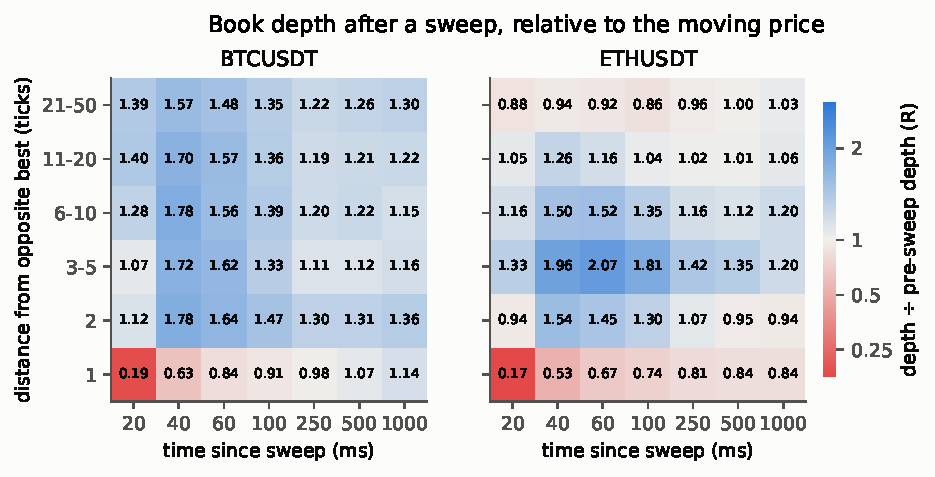
\includegraphics[width=\textwidth]{figures/fig3_recovery_heatmap.pdf}
\caption{Swept-side depth relative to pre-sweep depth, by distance from the opposite best quote
(rows) and time since the sweep (columns). Ratio of sums over clean sweeps.}
\label{fig:heat}
\end{figure}

\subsection{Mass balance: depth falls before it rises}
Table~\ref{tab:kappa} and Figure~\ref{fig:kappa} report $\kappa$. In the first 100\,ms after a
sweep, cancellations exceed additions on the swept side (BTC $\kappa = 0.74$ at 20--40\,ms;
ETH 0.61), whereas matched placebo times show balanced churn ($\kappa \approx 1.00$--$1.07$).
Additions exceed cancellations by more than at placebo times only from 100--250\,ms (ETH) or
250--1000\,ms (BTC) onward.

\begin{table}[ht]
\centering
\caption{Added $\div$ cancelled swept-side depth ($\kappa$) by window after the sweep. 95\%
day-cluster bootstrap intervals in brackets. Placebo: state-matched.}
\label{tab:kappa}
\begin{tabular}{lcccc}
\toprule
 & \multicolumn{2}{c}{BTCUSDT} & \multicolumn{2}{c}{ETHUSDT} \\
\cmidrule(lr){2-3}\cmidrule(lr){4-5}
Window (ms) & Sweeps & Placebo & Sweeps & Placebo \\
\midrule
20--40    & 0.74 [0.68, 0.80] & 1.05 & 0.61 [0.56, 0.66] & 1.01 \\
40--100   & 0.87 [0.82, 0.91] & 1.07 & 0.85 [0.81, 0.89] & 1.00 \\
100--250  & 0.99 [0.95, 1.02] & 1.04 & 1.12 [1.08, 1.16] & 1.03 \\
250--1000 & 1.11 [1.09, 1.12] & 1.04 & 1.09 [1.07, 1.11] & 1.03 \\
\bottomrule
\end{tabular}
\end{table}

\begin{figure}[ht]
\centering
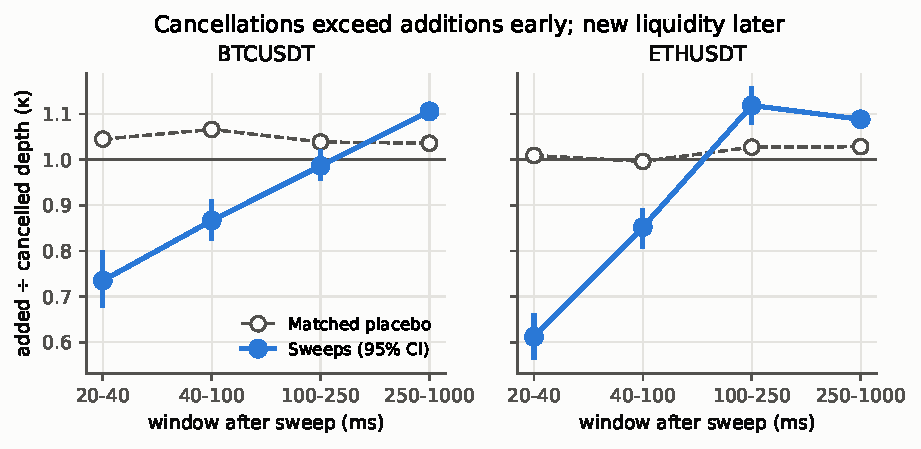
\includegraphics[width=\textwidth]{figures/fig2_mass_balance.pdf}
\caption{Added $\div$ cancelled swept-side depth after sweeps (filled, 95\% CI) and at
state-matched placebo times (open). Values below 1: depth is removed faster than it is added.}
\label{fig:kappa}
\end{figure}

\subsection{Three phases}
Table~\ref{tab:phases} and Figure~\ref{fig:phases} report the decomposition.

\begin{table}[ht]
\centering
\caption{Three-component decomposition of post-sweep flows (excess over matched placebo,
fractions of pre-sweep swept-side depth). Deep book: $d>5$. 95\% day-cluster bootstrap
intervals in brackets.}
\label{tab:phases}
\begin{tabular}{lcc}
\toprule
 & BTCUSDT & ETHUSDT \\
\midrule
Withdrawal, $<250$\,ms        & 0.22 [0.18, 0.25] & 0.20 [0.17, 0.25] \\
Repositioning, $<250$\,ms     & 0.19 [0.16, 0.21] & 0.09 [0.07, 0.11] \\
Source, $<250$\,ms            & 0.01 [0.00, 0.02] & 0.02 [0.02, 0.03] \\
Source, $>250$\,ms            & 0.21 [0.17, 0.23] & 0.12 [0.09, 0.14] \\
Repositioning share of near-touch build-up, $<250$\,ms & 0.93 [0.89, 0.97] & 0.81 [0.73, 0.86] \\
Centroid: withdrawal (ms)     & 69 & 47 \\
Centroid: repositioning (ms)  & 322 & 133 \\
Centroid: source (ms)         & 507 & 449 \\
\bottomrule
\end{tabular}
\end{table}

\begin{figure}[ht]
\centering
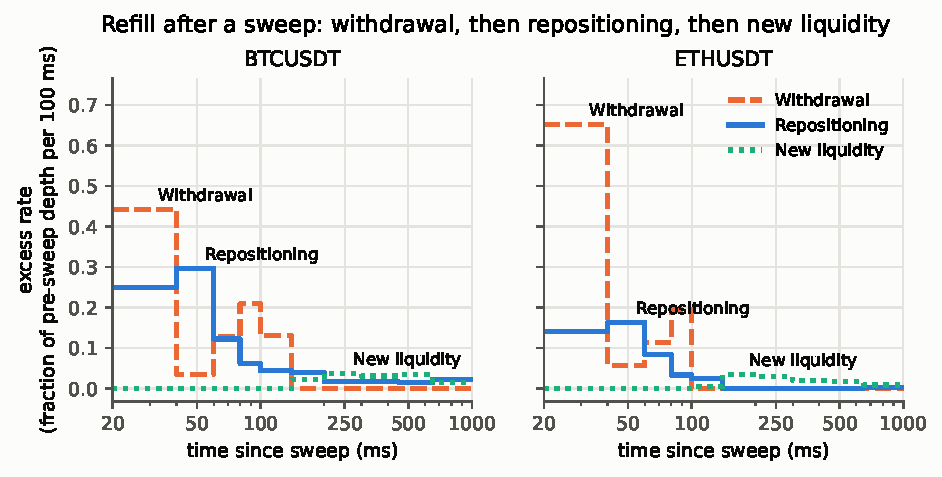
\includegraphics[width=\textwidth]{figures/fig1_three_phases.pdf}
\caption{Excess rates of withdrawal, repositioning and new liquidity after a sweep. Rates are
per 100\,ms; the late source is spread over a long interval, so its integrated mass
(Table~\ref{tab:phases}) is comparable to early repositioning.}
\label{fig:phases}
\end{figure}

Restricting the deep book to $6\leq d\leq 50$ shrinks BTC withdrawal from 0.22 to 0.04 (most of
it is cancellation of orders stranded more than 50 ticks from the new price) but leaves the
ordering and the dominance of repositioning before 250\,ms intact (share 0.74 [0.66, 0.83] BTC;
0.78 [0.73, 0.84] ETH).

%----------------------------------------------------------------------------------------------
\section{Implications for continuum models}

Write $\rho(x,t)$ for swept-side depth at distance $x$ from the opposite quote. A local
reaction--diffusion description, $\partial_t\rho = D\,\partial_x^2\rho - \nu\rho + \lambda(x)$,
refills a cleared region from its edges. Our evidence instead supports
\begin{equation}
  \partial_t \rho(x,t) = \int K(x,y,t)\,[\rho(y,t) - \rho(x,t)]\,dy \;-\; \nu(x,t)\,\rho(x,t) \;+\; S(x,t),
\end{equation}
with a non-local kernel $K$ active within the first few hundred milliseconds (repositioning), a
state-dependent cancellation rate $\nu$ that spikes immediately after the shock (withdrawal),
and a delayed source $S$ centred near half a second. We do not detect a local diffusion
component at these horizons. \todo{estimate $K$, $\nu(t)$, $S(t)$ parametrically; Knudsen-number
check of continuum validity \citep{yura2015knudsen}.}

%----------------------------------------------------------------------------------------------
\section{Related literature}
\todo{expand from docs/literature\_review.md: resilience
\citep{large2007resiliency,degryse2005aggressive,xu2017resiliency,clapham2021speed,lo2015resiliency};
continuum and SPDE models
\citep{donier2015minimal,mastromatteo2014anomalous,cont2021spde,hambly2024porous,benzaquen2018fractional,diana2024anomalous};
point processes \citep{bacry2015hawkes,lu2018highdim,rambaldi2017volume,huang2015queue};
cancellations and quote fade \citep{MalinovaPark2016,hasbrouck2009fleeting}; placement inside the
spread after liquidity crises \citep{ponzi2006crises}; crypto perpetual microstructure
\citep{albers2025dilemma}.}

%----------------------------------------------------------------------------------------------
\section{Robustness and limitations}
\begin{itemize}
  \item \textbf{Level-2 data.} Without order identifiers we cannot show that the \emph{same}
        orders move; repositioning is identified from matched aggregate cancellation and
        addition flows.
  \item \textbf{Push netting.} Each 20\,ms message nets changes at a price, so gross flows are
        lower bounds.
  \item \textbf{Fill matching.} About one third of sweep volume exceeds the displayed size at
        its price (hidden or newly posted liquidity); matchable volume is capped at displayed
        size so it cannot absorb later cancellations.
  \item \textbf{Venue and assets.} One venue, two assets. \todo{SOLUSDT, XRPUSDT, LINKUSDT
        (Bybit) and Binance BTCUSDT futures.}
  \item \todo{robustness by sweep size, side, time of day; finer state matching.}
\end{itemize}

%----------------------------------------------------------------------------------------------
\section{Conclusion}
After a multi-level sweep, the crypto perpetual order book refills in three ordered phases:
liquidity is first pulled, then moved to the new price, and only then made anew. The sequencing
is invisible in aggregate resilience measures and in best-quote studies, and it is inconsistent
with diffusion-type continuum models at sub-second horizons. \todo{implications for execution
and market-making models.}

\bibliographystyle{plainnat}
\bibliography{references}

\end{document}
